\documentclass[twocolumn]{article}
\usepackage{subfig}
\usepackage{graphicx}
\begin{document}
	\title{\begin{titlepage}
			My paper
	\end{titlepage}}
	\section{1}
	\subsection{Intro to mav and control system architecture}
	Multirotor Aerial Vehicles (MAV), specifically quadrotors, have become quite commonplace in many industries ranging from filmography to racing to even military operations. Over the past decade, there has been an incredible amount of research and advancement within this field leading to its proliferation and allowing for the technology to become more accessible. One of the major areas of research regarding MAV's is the control system that directs the motor-rotor system. The control mechanism can be as simple as a motor-rotor control, all the way to controlling the torque, or thrust or one of many other variables. The control of the motor-rotor has to account for multiple different factors, from the ambient wind speed, the rotation, the pitch of the propeller, all the way to the high level control system of the ESC. \\
	In general, there are two different types of control loops; open and closed. Open control loops are what the majority of MAV control systems are. There is a flight controller, that sends a signal to the ESC that applies a particular voltage to the motor based on previously calibrated settings. In this method, the final result of the motor spinning is unknown to the flight controller. Therefore given any disturbances, there will be large variances in the response of the overall system. In response to these systems there are smarter, closed loop control. This is the type of control we will focus on. Closed loop systems provide a certain way to measure the output of the rotor based on the input from the FC. This allows for a smarter, more robust system and greater control of the output. \\
	\subsection{Intro to the problem}
	The main problem we are trying to answer is how to create an effective, efficient, and reasonable solution to having a closed loop control system. This would include having a type of sensor which would measure the thrust output of the propellor and relay that onto the ESC so that the ESC can control the thrust output accordingly.
	\subsection{1.3}
	\subsection{1.4}
	The scope of this paper is to introduce a wind sensor as an external sensor and develop the relationship between the downwash rotor wind speed and the thrust vector of the propeller. Doing that we can implement a control system by which the wind sensor can be used to maintain a thrust given disturbances or faults within the system. 
	\section{2}
	\subsection{Wind sensor math/theory}
	We have to start by defining the three different velocities that apply to a propeller.\\
	\begin{eqnarray}
	\label{e1}
	v_x , v_y , v_z \\
	\label{e2}
	v^s_{x} , v^s_{y} , v^s_{z} \\
	\label{e3}
	v^i_{x} , v^i_{y} , v^i_{z}
	\end{eqnarray}
	Where equation \ref{e1} Is the velocity of the drone, the body frame velocity, equation \ref{e2} is the velocity of the wind approaching the propellers, the stream velocity, and equation \ref{e3} is the induced velocity of the propellers.\\
	Since we are doing only the static tests, we do not have to worry about horizontal winds, so we can say 
	\begin{eqnarray}
	\nonumber
	v_s = v^s_{z}\\
	\nonumber
	v_i = v^i_{z}
	\end{eqnarray}
	As well, since we have stationary system, the frame velocities can be ignored as well. What the wind sensor will notice is 
	\begin{equation}
	v_{tot} = v_{i} + v_{s}
	\label{vtot}
	\end{equation}	
	Generally, when no disturbances are applied we can assume that $v_s$ is $0$ as a means of simplifying our system.
	
	Modern Device \cite{md} gives us the equation 
	\begin{eqnarray}
		WS = \frac{(V - V_{z})*0.087288}{3.038517 * T_{c} ^{0.115157}} ^ {3.009364}
		\label{wind_speed}
	\end{eqnarray}
	Where $WS$ is the wind speed,in miles/hour, $V$ is the measured voltage, $V$ is the calibrated voltage when there is no wind, and $T_c$ is the current temperature in celsius which is also measured by the sensor. While the basis of this paper is around the wind speed, it is not important to know the exact wind speed and therefore throughout the rest of our calculations, we only consider the measured voltage. 
	
	%How does wind speed relate to voltage
	
	To explain the relation of wind to thrust, let's radically simplify it and assume it is a linear system. For the first case let this be in a situation with no stream velocity, or $v_s = 0$. With this being the case, it can be stated that 
	\begin{equation}
	F_p= \frac{\partial p}{\partial t}
	\label{fvm}
	\end{equation}
	where $F_p$ is the force the propeller exerts, $p$ is momentum and $t$ is time. From this we can expand this to 
	\begin{equation}
	F_p= \frac{mv_{tot} - mv_{s}}{\Delta t} 
	\label{fvm2}
	\end{equation}
	where $m$ is the mass of air flowing. If we assume that this is over a 1 second time span we get
	\begin{equation}
	F_p= m*(v_{tot}-v{s}) 
	\label{fvm3}
	\end{equation}
	Now to consider the efficiency of the propeller we can say 
	\begin{eqnarray}	
	V_{i}\prime = V_{i}* \gamma\\
	V_{tot}\prime = V_i\prime + V_s
	\label{eff}
	\end{eqnarray}
	where $\gamma$ is some efficiency factor $0 < \gamma < 1$ which degrades as the stream velocity $v_s$ approaches $v_i$ \cite{someone}. In doing so we can assume that for a non-zero $v_s$ 
	\begin{equation}
	F_p\prime < F_p
	\end{equation}
	This is the reasoning behind why as winds buffett a drone mid-flight, the drone's thrust vector tends to drop. 
	\subsection{Kalman Math}
	\subsection{2.3}
	\subsection{2.4}
	
	\section{3}
	\subsection{Thrust stand}
	%THE THRUST STAND
	In our setup we used a thrust stand obtained from RCBenchmark, specifically the RCBenchmark Thrust stand and Dynamometer Series 1580 \cite{rcb} as our testbed. The measurements from the thrust stand will be our "ground truth". This thrust stand incorporates a micro-controller board along with three, three-axis strain guage to measure the forces and the torque derived by the propeller. The board also collects data on the voltage, current and the signal to the ESC's which allows us to measure the power draw of the motor, and the RPM of the motor. Along with this there is an associated GUI which allows us to control the board and collect and visualize the data. The testbed collects data at a very high rate of close to 1kHz but then averages the data to eliminate outliers, so the data rate is 40Hz. This is more than adequate for the purposes of modeling the thrust response of the propeller to various stimuli. 
	\subsection{Wind Sensor Intro}
	The wind sensor we have chosen to use is the "Modern Device- Wind Sensor Rev. P" \cite{md}. This device is a hot wire anemometer that is designed to measure wind from any direction. Hot wire anemometers work by passing a constant current through a thin wire which heats up due to the current. As the wind flows past the wire, the wire will be cooled down rapidly, resulting in a change in the measured voltage, which is the value that we observe \cite{hot_wire}. This system allows us to measure the wind speed that is resultant of the propeller. 
	\subsection{Wind Sensor Proof}
	To understand the limitations of the wind sensor, we performed a series of tests to characterize the sensor. The first of which was to determine under which orientation the sensor observed the highest range of wind speeds. As seen in \ref{orient_test}, the orientation of placing the wind sensor normal to the direction of wind flow allowed for the highest range of measurement. Next we performed a test to determine the feasible range of measurement. This was done by exposing the wind sensor to a step-signal test and a pulse signal test ranging from the minimal PWM value to approximately $50\%$ of the motor's max value, the results of which are in \ref{min_max}. The PWM values in this case are based around the Simulink-Arduino Library PWM module.  This resulted in a working range from $PWM = 44$ to $PWM = 60$. While there is possibility for the wind sensor to measure higher wind speeds, there is a significant amount of noise even with the addition of a low-pass filter, hence we decided to limit the max speed of our experiment. 
	
	Another factor that we deem is important to characterize is the speed of response to change of wind speed. We measured this by running the propeller at various different speeds, while tracking the thrust output on the testbed as our base measurement of response time and then comparing the response time to see the lag in response time. By doing this we found that there was a negligible lag time of less than $10 ms$, which is our resolution for each measurement.
	 
	Lastly we measured the location of the wind sensor in relation to the propellers. To do so we measured a semi-circle area behind the propeller to deem the location of highest wind sensitivity. Resulting in a map as seen in figure \ref{area}. 
	
	By characterizing the wind sensor, we can ensure that it is in the optimal configuration for us to collect data.
	
	\section{Results}
	
	\subsection{Experimental Setup- How we set up the kalman/Algorithm}
	\begin{figure}[b]
		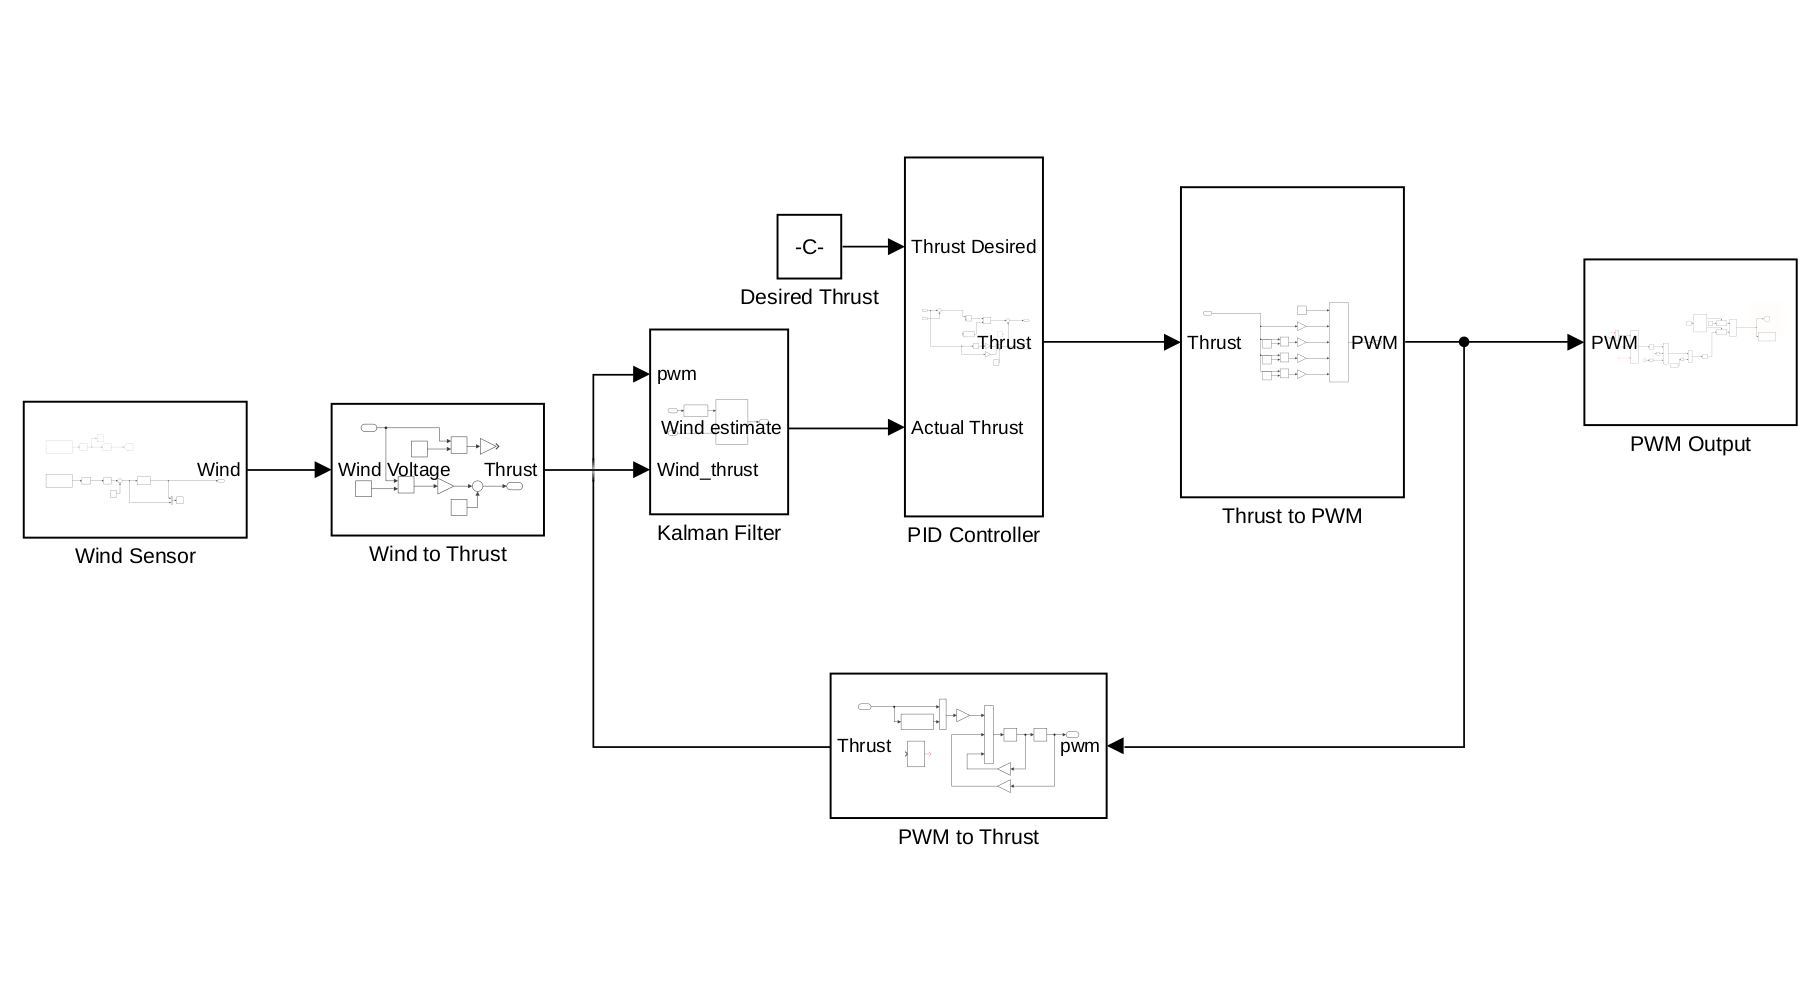
\includegraphics[width=\textwidth]{block_diagram}
		\caption{Block Diagram}
		\label{block_diagram}
	\end{figure}

	We developed a control architecture as pictured in fig \ref{block_diagram} where there are two sources of measurement for the thrust value. The first, main value, is from the wind sensor which is measured through an Arduino. The voltage value that the arduino measures is then converted to a thrust value through the power function
	\begin{equation}
	Thrust = 4.701 * 10^{15} * V_w^{6.146} + 0.0731
	\label{wind_power}
	\end{equation}
	
	The second measurement of thrust is a polynomial function that converts the recorded PWM value that is used to control the propeller to thrust. \newline
	\begin{eqnarray}
	Thrust = 1.957*10^{-5}*PWM^4 \\
	- 7.476*10^{-4}*PWM^3 \nonumber\\ 
	+ 1.272*10^{-2}*PWM^2 \nonumber\\
	+ .01092*PWM - .01842 \nonumber
	\label{pwm_poly}
	\end{eqnarray}
	
	These values are then passed through a Kalman Filter weighted for the wind sensor. This method allows for the system to accurately determine the thrust value output while reducing noise due to the nature of the wind. Next this value is passed to a PID controller which checks the current thrust value to the desired thrust value and outputs a thrust value. Lastly a polynomial function converts the thrust value back to PWM.
	\begin{eqnarray}
	PWM = -.1746*Thrust^4 + 1.008*Thrust^3\\ 
	- 3.409*Thrust*2 + 12.29*Thrust + 1.8430 \nonumber
	\label{pwm_poly}
	\end{eqnarray}
	\subsection{The tests}
	Once the characteristics of the wind sensor were determined we ran tests to ensure the viability of our algorithm and if it would respond to external stimuli the way we expected. The first test that we ran was to measure the response of the kalman filter and ensure that our thrust calculation was accurate in relation to the testbed recorded thrust. To do this we measured  As seen in fig \ref{kalman} the kalman filter, while noisy due to the wind variations in the wind sensor data, follows the thrust value from the testbed closely. This result gives us the confidence to setup the PID based on the kalman filter's value. 
	
	To ensure the functionality of the controller we set up several faults and disturbances to test the response of the system. The first step was to create an external disturbance by placing another propeller and blowing wind perpendicular to the axis of the main propeller. This would be akin to horizontal crosswind flow across the propeller.
	\begin{figure}
		\label{content...}
	\end{figure}
	 Based on the results of fig \ref{wind_disturb}, the control algorithm can determine the appropriate correction for such a disturbance through
	\begin{figure}
		content...
	\end{figure}
	Next we 
	\subsection{4.3}
	\subsection{4.4}
	
	\section{5}

	\subsection{5.1}
	\subsection{5.2}
	\subsection{5.3}
	\subsection{5.4}

	
	

	\begin{thebibliography}{99}
		\bibitem{Mahoney1} Mahoney 2012
		\bibitem{rcb} https://www.rcbenchmark.com/dynamometer-series-1580/
		\bibitem{md} https://moderndevice.com/product/wind-sensor-rev-p/
		\bibitem{hot_wire} Extended Applications of the Hot‐Wire Anemometer, Stanley Corrsin,Review of Scientific Instruments 1947 18:7, 469-471 
		
	\end{thebibliography}


\end{document}